\documentclass[runningheads]{llncs}
 
\usepackage{booktabs}
\usepackage[algo2e]{algorithm2e} 
\usepackage{graphicx}
\usepackage[misc]{ifsym}
\usepackage{xcolor}
\usepackage[normalem]{ulem}

\title{Biomarker Localization by Combining CNN Classifier and Generative Adversarial Network}
\titlerunning{Robustness}
\author{Rong Zhang\inst{1,2} \and Shuhan Tan\inst{1}\and Siyamalan Manivannan\inst{3} \and Ruixuan Wang \inst{1,2} \and Haotian Lin\inst{4} \and Jingjing Chen\inst{4}\and Wei-Shi Zheng\inst{1,2}}
% index{Zhang, Rong}
% index{Tan, Shuhan}
% index{Manivannan, Siyamalan}
% index{Wang, Ruixuan}
% index{Lin, Haotian}
% index{Chen, Jingjing}
% index{Zheng, Wei-Shi}
\authorrunning{R. Zhang \& S. Tan et al.}
\institute{School of Data and Computer Science, Sun Yat-sen University, China \and
	Key Laboratory of Machine Intelligence and Advanced Computing, MOE, Guangzhou, China \and
	Department of Computer Science, University of Jaffna, Sri Lanka\and
	Zhongshan Ophthalmic Center of Sun Yat-sen University, Guangzhou, China
	 \\
	\email{wangruix5@mail.sysu.edu.cn}}
\begin{document}

\maketitle

\newcommand{\shh}[1]{{\color{blue} #1}}

\begin{abstract}
This paper proposes a novel deep neural network architecture to effectively localize potential biomarkers in medical images, when only the image-level labels are available during model training. The proposed architecture combines a CNN classifier and a generative adversarial network (GAN)
in a novel way, such that the CNN classifier and the discriminator in the GAN can effectively help the encoder-decoder in the GAN to remove biomarkers. Biomarkers in abnormal images can then be easily localized and segmented by subtracting the output of the encoder-decoder from its original input. The proposed approach was evaluated on diabetic retinopathy images with real biomarkers and on skin images with simulated biomarkers, showing state-of-the-art performance in localizing biomarkers even if biomarkers are irregularly scattered and are of various sizes in images.
\end{abstract}

\begin{keywords}
Biomarker Localization, Encoder-Decoder, Generative Adversarial Networks.
\end{keywords}
\section{Introduction}

Visual biomarkers in medical images are important indicators for radiologists to investigate the risks, categories, and status of particular diseases. Therefore, automatic localization and segmentation of existing or potentially novel biomarkers from various medical images would be a key step for intelligent diagnosis and treatment of diseases. While it is relatively easier for human experts to roughly locate biomarkers (e.g., with bounding boxes surrounding biomarker regions), it is challenging, if not impossible, for humans to precisely localize and segment biomarkers particularly when they are irregularly scattered in images. As a result, it is highly desirable to precisely localize biomarkers only based on weak annotations, e.g., image-level labels representing whether images contain diseases (labelled `abnormal') or not (labelled `normal').

Multiple approaches have been proposed to alleviate the great challenge of biomarker localization only based on image-level annotations. One traditional approach is multiple instance learning~\cite{maron1998framework}, a weakly supervised technique which can train a classifier not only predicting the labels of images, but also roughly localizing the discriminative regions (possible biomarkers) in abnormal images. Such technique has been applied to solve various medical imaging problems, such as segmenting retinal nerve fibers from retinal fundus images~\cite{Manivannan} and  cancer detection in digital pathology images~\cite{Melih}. Another group of approaches, proposed in the computer vision community, is through visualizing image regions on which convolutional neural network (CNN) classifiers focus when predicting classes of images. Among them, perturbation methods occlude or mask each possible local region and check the changes in classifier outputs, with larger drops in output indicating higher importance in predicting image classes~\cite{zintgraf2017visualizing}. 
%fong2017interpretable,zeiler2014visualizing
In comparison, feature activation methods locate important local regions based on activated regions in feature maps of certain convolutional layer's output, e.g., the popular class activation mapping (CAM)~\cite{zhou2016learning} and its variants Grad-CAM~\cite{selvaraju2017grad} etc.
%CAM with Dilated Convolutions \cite{Wei_2018_CVPR}  
Recently, the CAM-based methods have been widely applied in medical image analyses, e.g., for pneumonia detection on chest X-ray images~\cite{rajpurkar2017chexnet}, bladder cancer prediction in digital pathology images~\cite{zhang2017mdnet} and Alzheimer diagnosis in MRI images~\cite{yang2018visual}.
%,breast cancer prediction in ultrasound images\cite{wu2018expert} and lesion segmentation in retinal \cite{Gondaletal17}
%and skin \cite{jia2017skin} images
However, all the above methods can only roughly locate biomarker or lesion regions, leaving the precise localization of biomarkers as an open problem.
%digital pathology images\cite{graziani2018visual}

In this paper, to precisely localize biomarkers, we propose a deep neural network architecture by combining a CNN classifier, a generator and a discriminator. The generator aims to output a normal version of each abnormal input image by removing potential biomarkers from the input image, such that the biomarkers in abnormal images can be easily localized and segmented by subtracting the output of the generator from its input. To help achieve this goal, a CNN classifier is added to encourage biomarker removal by classifying the subtraction (of the output of the generator from its input) as normal or abnomal. On the other hand, to make the output of the generator realistically normal, a discriminator is added and trained adversarially to discriminate real and generated normal images. Note that the generator and discriminator naturally form a generative adversarial network (GAN)~\cite{goodfellow2014generative}. 
Qualitative and quantitative evaluations on diabetic retinopathy images with real biomarkers and on skin images with simulated biomarkers showed superior performance of the proposed architecture to that of the CAM-based methods in precisely localizing biomarkers. 

\section{Method}\label{sec:method}
The purpose is to precisely localize potential biomarkers or lesion regions in abnormal images when only the image-level labels are available. Different from the visualization methods (e.g., CAM or Grad-CAM) which can only approximately localize potential biomarkers at low resolution in images after training a classifier, the motivation of our idea is to design a new architecture which can  learn to directly find precise locations of potential biomarkers. With this motivation, we proposed a novel deep neural network by combining two different learning architectures (Figure~\ref{fig1}): a supervised CNN classifier and a GAN (composed of an encoder-decoder and a discriminator).  

In the proposed architecture, the encoder-decoder network tries to remove any potential biomarkers from the input image, generating a fake normal image for abnormal input image, or keeping the output image the same as the input if the input is normal. By subtracting the output of the encoder-decoder from its input, any biomarkers can be easily localized and segmented. While it is possible to train such an encoder-decoder just with normal images, this does not make use of the existing abnormal images, therefore not directly learning biomarker features for localization. Instead, to more effectively achieve the goal of the encoder-decoder, a CNN classifier is added on top of the encoder-decoder, with input being the subtraction of the encoder-decoder's output from its input, and expected output being the label of the original input image to the auto-encoder. In order to accurately classify images, the CNN classifier together with the encoder-decoder would have to differentiate abnormal images from normal ones. Ideally, if the input to the classifier contains only biomarkers for abnormal original images and contains nothing (zero values everywhere) for normal images, the classifier would more easily and accurately predict the category of the original images. In other words, training a more accurate classifier could help the encoder-decoder's output keep the normal regions and remove biormakers from the original image, such that the input to the classifier only contains biomarker signals.

However, the classifier may help localize just part of biomarkers from the original images. This is because localizing part of biomarker signals from original abnormal images (and localizing little signal from normal images) is enough for the classifier to easily differentiate between normal and abnormal images. In this case, the encoder-decoder output would still contain some biomarkers.

To further help the encoder-decoder remove potential biomarkers from original (abnormal) images, a discriminator is added to judge whether the output of the encoder-decoder looks like a real normal image or not. By forcing the encoder-decoder's outputs to look more like normal images, the discriminator helps the encoder-decoder remove as much biomarker signals as possible from original images. 

\begin{figure}[tbp]
	
	% \vspace{-2cm}
    \centering
    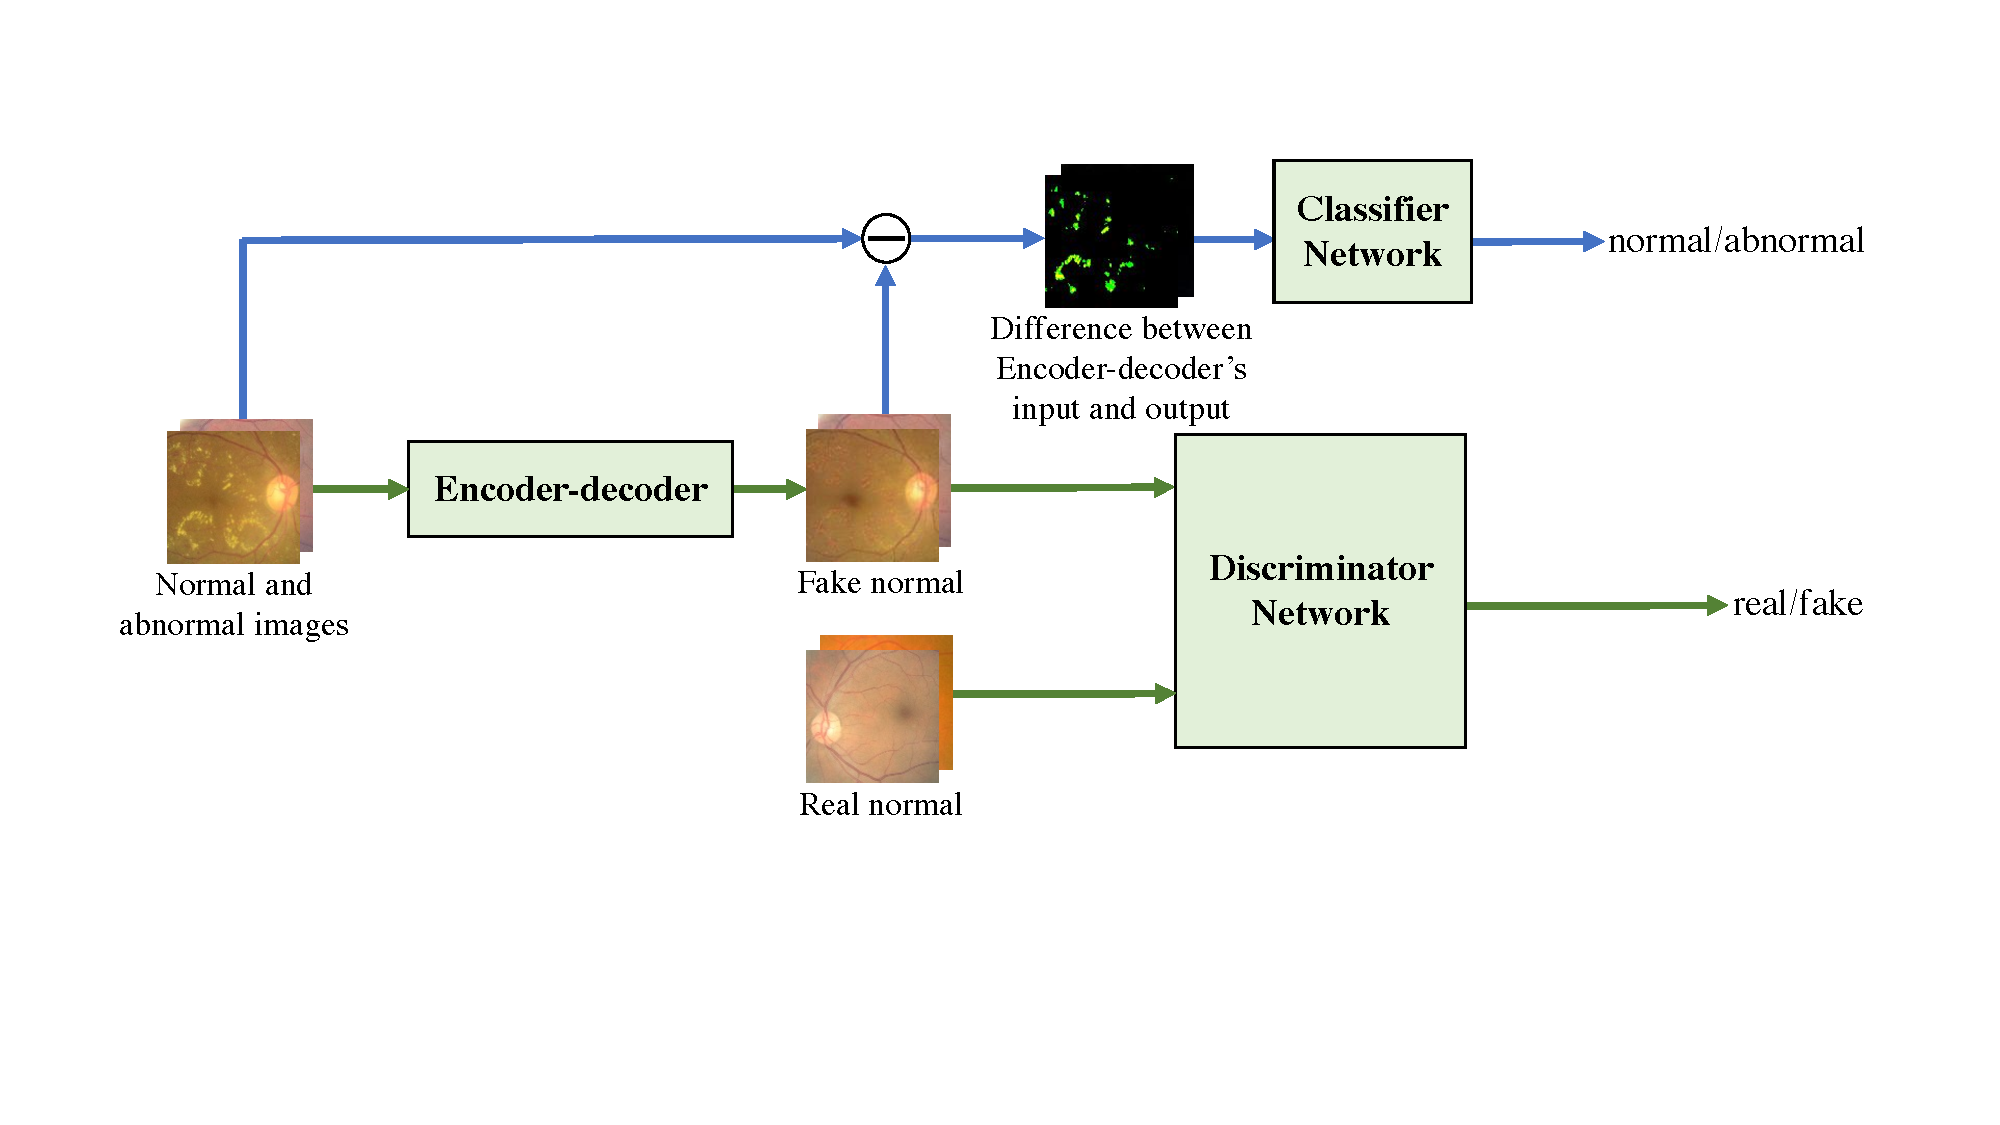
\includegraphics[width=1.0\linewidth]{images/method} 
    \caption{The proposed architecture for biomarker localization. The classifier and the discrminator together can help the encoder-decoder more effectively remove biomarkers from input images. Biomarkers can then be localized by subtracting the encoder-decoder's output from its input.}\label{fig1}
    \vspace{-0.5cm}
\end{figure}
It is clear that the encoder-decoder and the discriminator together form a generative adversarial network (GAN). One may consider that the GAN itself, without the classifier component in the architecture, may be enough to help the encoder-decoder remove potential biomarkers from images. However, GAN itself could help too much such that, although the encoder-decoder generates quite normal images, the normal regions of the encoder-decoder's output may also be changed compared to the input. In this case, the subtraction of the encoder-decoder's output from its input, i.e., the input to the classifier, would contain both normal and biomarker signals, which in turn makes it relatively more difficult for the classifier to differentiate abnormal images from normal ones. That means, the classifier and the discriminator should work together to help the encoder-decoder remove potential biomarkers, i.e., the discriminator helps the encoder-decoder output normal images and the classifier helps the encoder-decoder only change biomarker regions to generate normal outputs. This has been experimentally confirmed (see Section~\ref{subsec:roles_of_architecture_components}).

In the proposed architecture, let us denote the encoder-decoder by $G$, the discriminator by $D$, and the classifier by $C$, then the problem of biomarker localization can be formulated as optimizing the deep neural network model by 
\begin{equation} 
\min_{G, C} \max_D \;\; L_{GAN}(D,G) + \lambda_1 L_{CE}(C,G) + \lambda_2 L_{ED}(G),
\end{equation}
where $L_{GAN}(D,G)$ is the objective function of the GAN (here we used WGAN; \cite{arjovsky2017wasserstein}), $L_{CE}(C,G)$ is the cross-entropy loss for the classifier $C$, and $L_{ED}(G)$ is the encoder-decoder loss (here we used $L1$ loss) emphasizing the similarity between its output and input. $\lambda_1$ and $\lambda_2$ are coefficients balancing the three different parts.

During model training, an alternating  strategy is adopted by updating different parts of the model iteratively, i.e.,
\begin{equation}
\min_{G, C} \;\; L_{1}=\lambda_1 L_{CE}(C,G) + \lambda_2 L_{ED}(G),
\end{equation}
\begin{equation}
\min_{G} \max_D \;\; L_{2}= L_{GAN}(D,G) + \lambda_2 L_{ED}(G).
\end{equation}


\section{Experimental Evaluation}
\subsection{Experimental settings}
Two datasets were used to evaluate the proposed model. One was derived from the Kaggle Diabetic Retinopathy (DR) dataset \footnote{\url{https://www.kaggle.com/c/diabetic-retinopathy-detection/data}}, from which 2,101 abnormal images containing clear diabetic biomarkers and 2,101 normal images were selected. Uninformative dark regions in each image were removed before inputting to the neural network. Since it is highly costly for humans to precisely locate and segment the biomarkers in all abnormal images, here 40 abnormal images were randomly selected and then annotated at pixel level by two practising ophthalmologists. Note that the pixel-level annotations were not for model training but only for quantitative evaluation of the proposed model on the DR dataset. 

The second dataset consists of skin images with artificial biomarkers. To generate this dataset, 2,920 normal images (actually image patches) of size $128\times 128$ were firstly extracted from a dermoscopy image dataset \cite{codella2018skin}. To simulate varying number, size, and location of biomarkers in real skin images, the values of these parameters were randomly generated in a certain range for each simulated skin image. More specifically, for each image of the half dataset, one to three images were randomly selected from the ImageNet~\cite{deng2009imagenet} and resized to either $4\times 4$, $8\times 8$ or $16 \times 16$ pixels. The thumbnail images were embedded into the skin image and then locally smoothed as artificial biomarkers. Pixel-level annotations were available for all artificial biomarkers.
 
In the proposed architecture, a modified UNet \cite{ronneberger2015u} was selected for the encoder-decoder network, with Tanh activation function added at last layer to constrain the pixel values of the UNet's output within the same range ([-1,1]) as that of the UNet's input. The UNet is pre-trained with all images for each dataset. A Resnet-18 was used for the classifier network and a seven-layer CNN for the discriminator network. Gradient penalty coefficient $\eta$ in the WGAN loss was set to 10. Adam was used for model training, with default learning rate=0.0002, batch size=32. For all tests, $\lambda _1=0.4$ and $\lambda _2=10.0$. We use PR curves for quantitative evaluation, which were generated by comparing the pixel-level localization results with ground truth annotations. The heat maps of localization results were normalized to [0,1] before PR generation. Please note that ROC curves are not suitable for evaluating the biomarker localization performance, as the proportions of positive and negtive pixels in each dataset are highly imbalanced (1:56 for DR dataset, 1:88 for skin dataset). Therefore, we only included the ROC curves for each experiment in the supplimentary material.   

Please note that our goal is to search for and localize visual (pixel-level) biomarkers from images with the help of image-level labels, rather than training a model to find biomarkers from new images. Therefore, for each dataset, all the images were used to train our model, and the model was then evaluated qualitatively and quantitatively. Thus we trained and evaluated our model on the same dataset.

\begin{figure}% [tbp]
	\centering
	% \vspace{-2cm}
	\includegraphics[width=1.0\textwidth]{images/u_d_c_comparation.pdf}
	\caption{Localization of biomarkers in retinal images. From left to right: original images, encoder-decoder output without the discriminator, the difference between first and second column, encoder-decoder output without the classifier, the difference between first and fourth column, encoder-decoder output with both classifier and discriminator included, the difference between first and sixth column.} \label{fig:model_components}
	\vspace{-0.5cm}
\end{figure} 

\subsection{Roles of architecture components}\label{subsec:roles_of_architecture_components}
This section evaluates the role of the classifier network and the discriminator network in the proposed architecture in localizing biomarkers from retinal images. We first compared the qualitative results. Figure~\ref{fig:model_components} shows that, without the discriminator, the classifier helped localize only part of the biomarkers ($3^{rd}$ column), leaving most of biomarkers remained in the output of the encoder-decoder ($2^{nd}$ column). On the other hand, without the classifier, the discriminator localized most (if not all) biomarker regions ($5^{th}$ column). However, some normal regions were also altered (red boxes in $4^{th}$ column), causing some false biomarkers including some regions along vessels (see localized vessel curves in $5^{th}$ column). In comparison, the combination of the classifier and the discriminator in the proposed approach resulted in the precise localization of most biomarkers, with much fewer false biomarkers ($7^{th}$ column) and biomarkers removed in the output of the encoder-decoder ($6^{th}$ column).  These results suggest that the classifier and the discriminator networks together help localize biomarkers as discussed in Section~\ref{sec:method}. This is further confirmed by quantitative evaluation of different model components, which shows that the proposed architecture (green `G-D-C' curve in Figure~\ref{fig:model_components_auc}) performs better than that without the classifier (blue `G-D' curve) or without the discriminator (red `G-C' curve). 

\begin{figure}%[bhp]
	% \vspace{-0.3 cm}
	\centering
	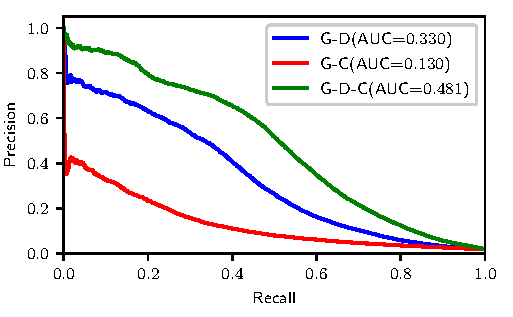
\includegraphics[width=.6\textwidth]{images/u_d_u_c_u_d_c_components}  
	\caption{Effect of model components. G-D represents encoder-decoder with only the discriminator, G-C represents encoder-decoder with only the classifier, and G-D-C represents our full model. The performance of the only encoder-decoder model was also evaluated, with AUC=0.083 only (not shown in figure). The PR curves were generated as decsribed in Section 3.1.
	} \label{fig:model_components_auc}
	\vspace{-0.5cm}
	%\vspace{-0.7cm}
\end{figure}

\subsection{Comparison with visualization methods for localization}
In this section we compare the localization ability of the proposed approach with the widely used visualization techniques CAM and Grad-CAM. ResNet-18 and VGG-19 binary classifiers were trained for CAM and Grad-CAM respectively.  As can be seen from Figure~\ref{fig:visual} (Left), while CAM found most biomarker regions, it also considered surrounding areas as part of biomarkers. This is largely due to the upsampling of the output of the last convolutional layer ($4\times 4$) to the image size ($128\times 128$). CAM also failed to detect most of the abnormal areas in the first image($3^{nd}$ column, $1^{st}$ row). As an extension of CAM,  Grad-CAM allows us to generate visual explanations from multiple layers, e.g., the intermediate convolutional layer ($4^{th}$ column, denoted as Grad-CAM-1) and the last convolutional layer ($5^{th}$ column, denoted as Grad-CAM-2). Although relatively accurate localization of biomarkers is attained in the $4^{th}$ column by Grad-CAM, the results are still either not precise ($1^{st}$ row) or not accurate ($2^{nd}$ and $3^{rd}$ row) enough. In comparison, the proposed approach gave much more precise localization of biomarkers with irregular shapes and scattered distributions, proving its superior performance to that of CAM and Grad-CAM. This is confirmed by  quantitative evaluation of each method (Figure~\ref{fig:visual}, Right), with the area under the PR curve (AUC) being 0.481 for the proposed model, 0.065 for CAM, and 0.061, 0.042 for different layers of Grad-CAM.


\begin{figure}%[tbp]
\centering 
\vspace{-0.5cm}
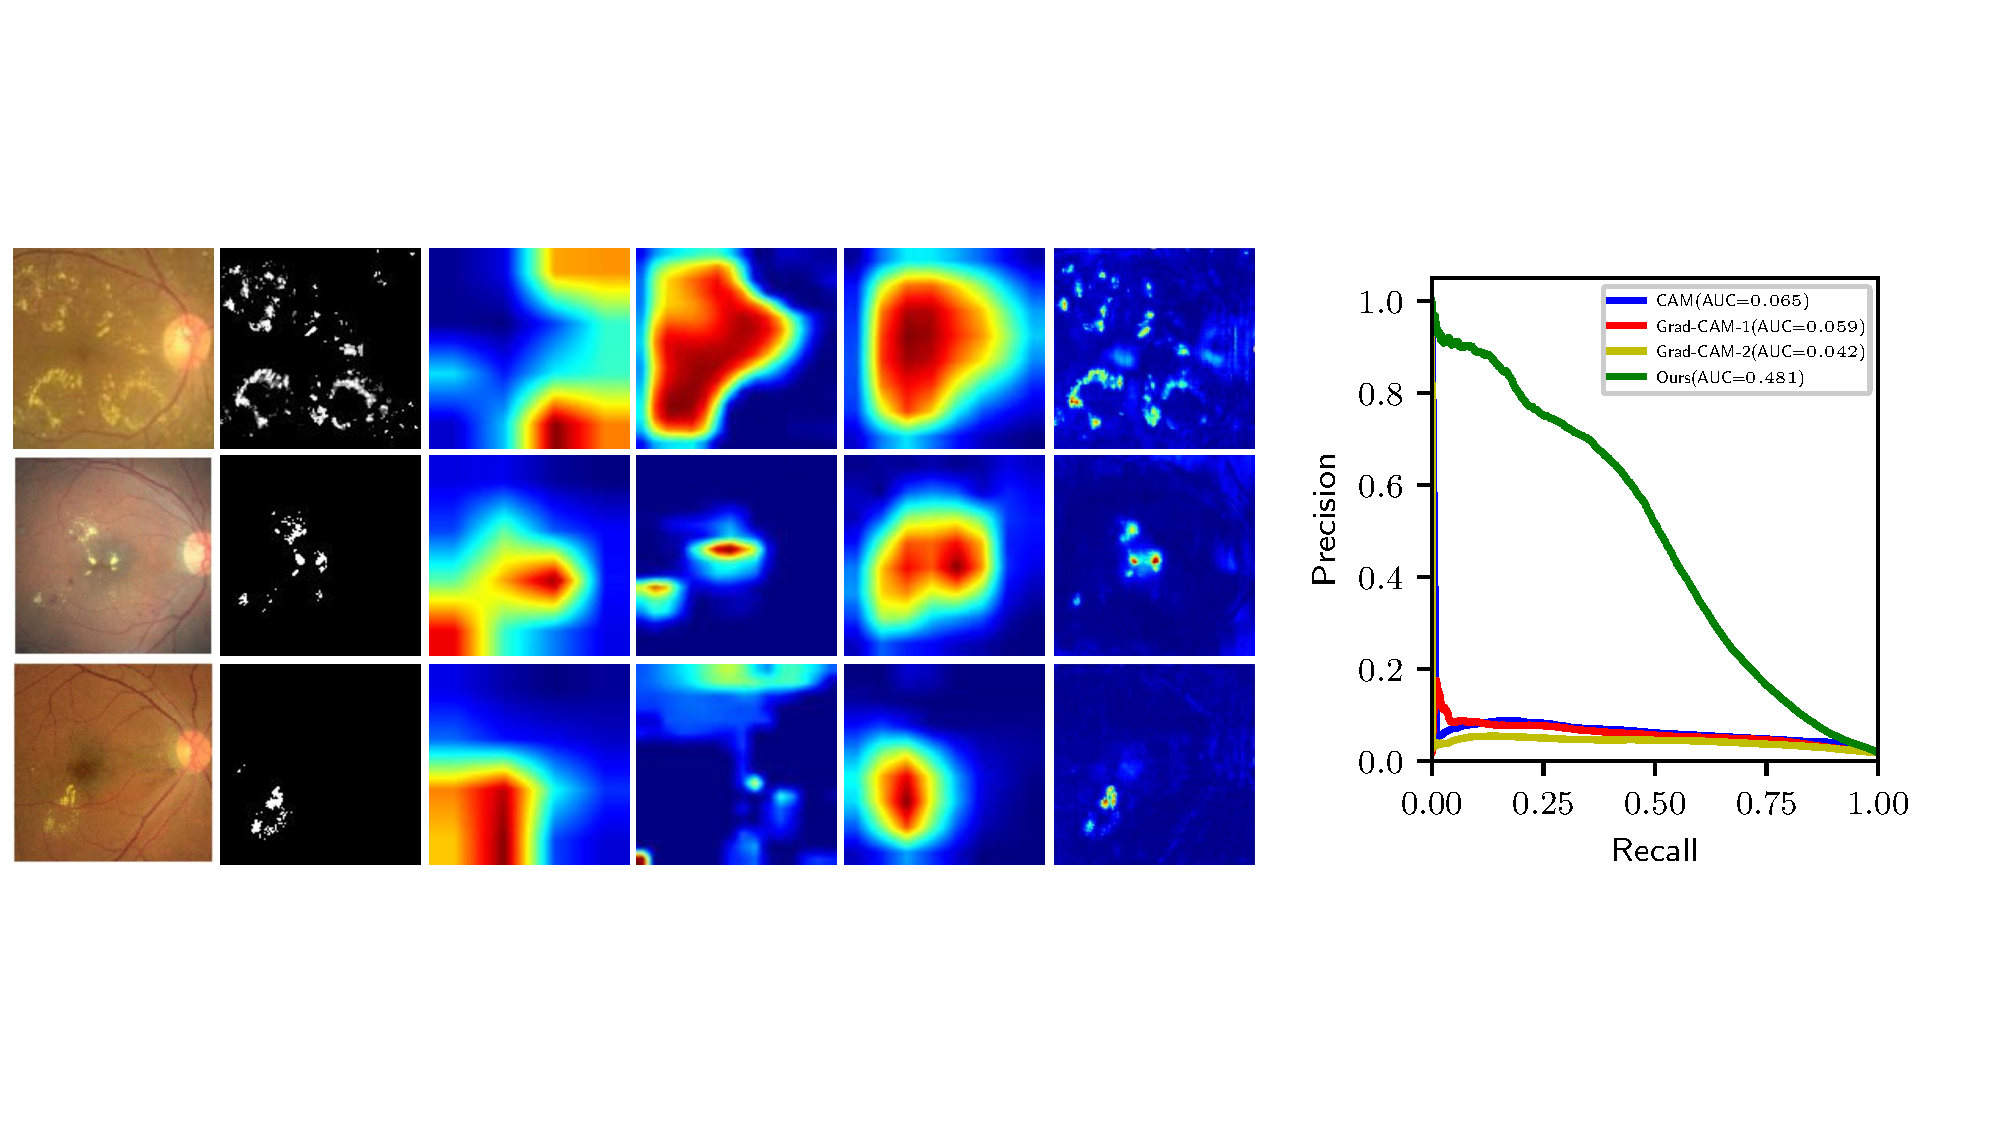
\includegraphics[width=0.95\linewidth]{images/retinal_image_pr.pdf}  
\caption{Comparisons with visualization methods on real diabetic retinopathy dataset. Left-half: localization results by CAM ($3^{rd}$ column), Grad-CAM-1 ($4^{th}$ column), Grad-CAM-2 ($5^{th}$ column) and our approach ($6^{th}$ column) on exemplar retinal images ($1^{st}$ column). Red regions in the heatmaps indicate higher probabilities to be biomarkers and blue for normal regions. The binary ground truth annoations are shown in the $2^{nd}$ column. Right half: the PR curve for each method. }\label{fig:visual} 
\vspace{-0.5 cm}
\end{figure}

The superior performance of the proposed model was further confirmed on the skin images with artificial biomarkers. Figure~\ref{fig:skin_eval} (Left half) shows that the proposed approach can almost perfectly and precisely localize the artificial biomarkers, while CAM and Grad-CAM again demonstrated inferior performance, with Grad-CAM better than CAM in localization. Figure~\ref{fig:skin_eval} (Right) confirms that our model is better (AUC=0.397) than CAM (AUC=0.075), Grad-CAM-1 (AUC=0.146) and Grad-CAM-2 (AUC=0.009). Note that in all tests, the classification performance of the classifiers are similar (above 97\% on both datasets), removing the potential influence of classification performance on biomarker localization.

\begin{figure} %[htb]
    \vspace{-0.5cm} 
	\centering 
	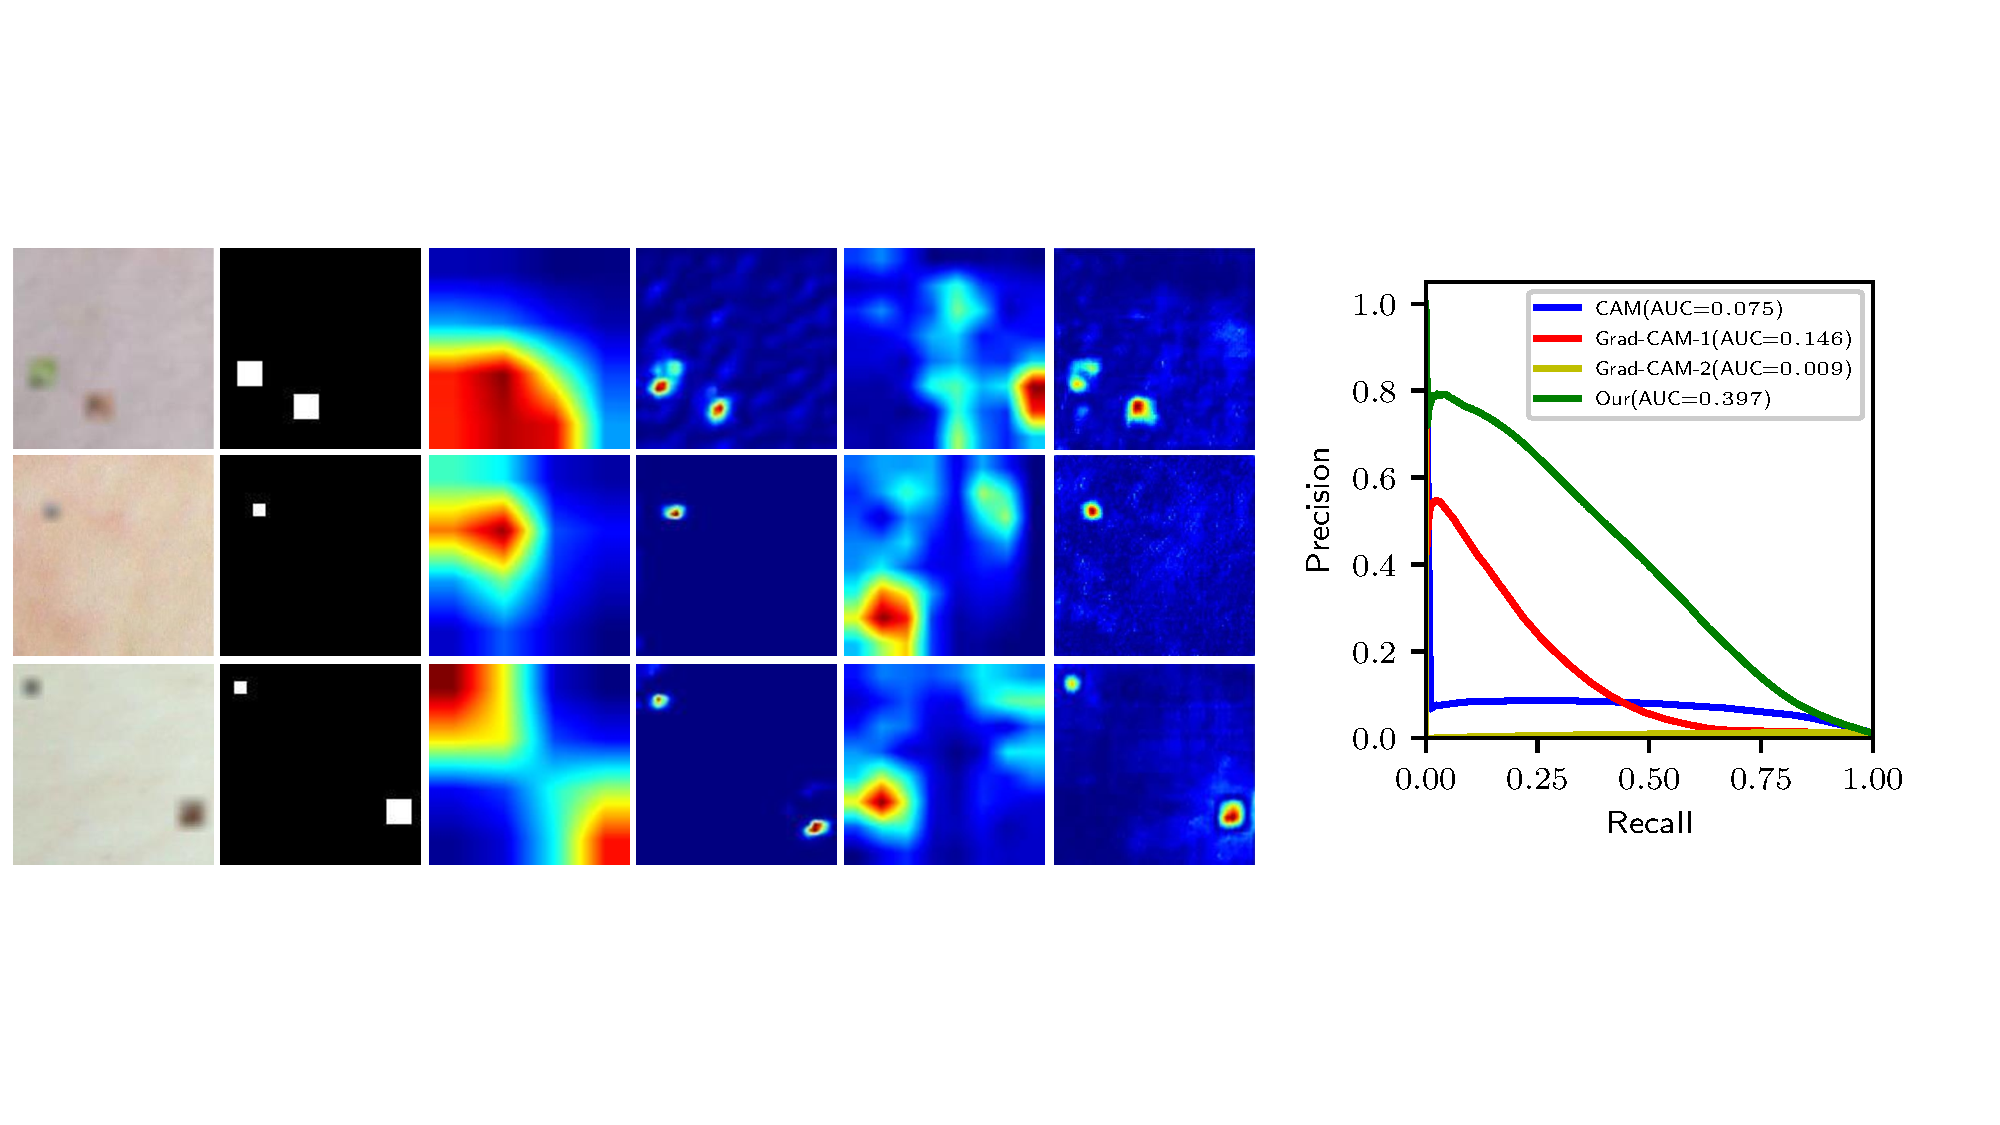
\includegraphics[width=0.95\textwidth]{images/skin_image_pr.pdf}
	\caption{Comparisons with visualization methods on skin image data. Left half: exemplar skin images ($1^{st}$ column), binary ground truth segmentation ($2^{nd}$ column), localization results by CAM ($3^{rd}$ column), Grad-CAM-1 ($4^{th}$ column), Grad-CAM-2 ($5^{th}$ column), and our approach ($6^{th}$ column). Right half: the PR curve for each method.}
	\label{fig:skin_eval}
	\vspace{-1.0cm}
\end{figure}


\section{Conclusion}
In this paper, a new deep neural network architecture fusing a CNN classifier and GAN together was introduced to effectively localize biomarkers from medical images. Compared with widely used localization methods, the proposed model can more precisely localize potential biomarkers even if they are irregularly scattered and of various forms and sizes. This provides a new way to detect potentially novel biomarkers for various diseases, which will be investigated as future work. 

~\\

\noindent\textbf{Acknowledgement.} This work is supported in part by the National Key Research and Development Program (grant No. 2018YFC1315402, No. 2018YFC0116500), the Guangdong Key Research and Development Program (grant No. 2019B020228001), and the National Natural Science Foundation of China (grant No. 81770967, No. 91846109).


\bibliographystyle{splncs04} 
% \bibliography{reference}
\begin{thebibliography}{10}
	\providecommand{\url}[1]{\texttt{#1}}
	\providecommand{\urlprefix}{URL }
	\providecommand{\doi}[1]{https://doi.org/#1}
	
	\bibitem{arjovsky2017wasserstein}
	Arjovsky, M., Chintala, S., Bottou, L.: Wasserstein {GAN}. arXiv preprint
	arXiv:1701.07875  (2017)
	
	\bibitem{codella2018skin}
	Codella, N.C., Gutman, D., et~al.: {Skin lesion analysis toward melanoma
		detection: A challenge at the 2017 international symposium on biomedical
		imaging (ISBI), hosted by the international skin imaging collaboration
		(ISIC)}. In: ISBI (2018)
	
	\bibitem{deng2009imagenet}
	Deng, J., Dong, W., Socher, R., Li, L.J., Li, K., Fei-Fei, L.: Imagenet: A
	large-scale hierarchical image database. In: CVPR (2009)
	
	\bibitem{goodfellow2014generative}
	Goodfellow, I., Pouget-Abadie, J., Mirza, M., Xu, B., Warde-Farley, D., Ozair,
	S., Courville, A., Bengio, Y.: Generative adversarial nets. In: NIPS (2014)
	
	\bibitem{Melih}
	Kandemir, M., Zhang, C., Hamprecht, F.A.: Empowering multiple instance
	histopathology cancer diagnosis by cell graphs. In: MICCAI (2014)
	
	\bibitem{Manivannan}
	Manivannan, S., Cobb, C., Burgess, S., Trucco, E.: Subcategory classifiers for
	multiple-instance learning and its application to retinal nerve fiber layer
	visibility classification. IEEE TMI  36(5),  1140--1150 (2017)
	
	\bibitem{maron1998framework}
	Maron, O., Lozano-P{\'e}rez, T.: A framework for multiple-instance learning.
	In: NIPS (1998)
	
	\bibitem{rajpurkar2017chexnet}
	Rajpurkar, P., Irvin, J., Zhu, K., et~al.: Chexnet: radiologist-level pneumonia
	detection on chest x-rays with deep learning. arXiv preprint arXiv:1711.05225
	(2017)
	
	\bibitem{ronneberger2015u}
	Ronneberger, O., Fischer, P., Brox, T.: U-net: convolutional networks for
	biomedical image segmentation. In: MICCAI (2015)
	
	\bibitem{selvaraju2017grad}
	Selvaraju, R.R., Cogswell, M., Das, A., Vedantam, R., Parikh, D., Batra, D.,
	et~al.: {Grad-CAM}: visual explanations from deep networks via gradient-based
	localization. In: ICCV (2017)
	
	\bibitem{yang2018visual}
	Yang, C., Rangarajan, A., Ranka, S.: Visual explanations from deep {3D}
	convolutional neural networks for {A}lzheimer's disease classification. arXiv
	preprint arXiv:1803.02544  (2018)
	
	\bibitem{zhang2017mdnet}
	Zhang, Z., Xie, Y., Xing, F., McGough, M., Yang, L.: Mdnet: a semantically and
	visually interpretable medical image diagnosis network. In: CVPR (2017)
	
	\bibitem{zhou2016learning}
	Zhou, B., Khosla, A., Lapedriza, A., Oliva, A., Torralba, A.: Learning deep
	features for discriminative localization. In: CVPR (2016)
	
	\bibitem{zintgraf2017visualizing}
	Zintgraf, L.M., Cohen, T.S., Adel, T., Welling, M.: Visualizing deep neural
	network decisions: prediction difference analysis. arXiv preprint
	arXiv:1702.04595  (2017)
	
\end{thebibliography}

\end{document}